\chapter*{Dodatak: Prikaz aktivnosti grupe}
		\addcontentsline{toc}{chapter}{Dodatak: Prikaz aktivnosti grupe}
		
		\section*{Dnevnik sastajanja}
		
		\textbf{\textit{Kontinuirano osvježavanje}}\\
		
		 \textit{U ovom dijelu potrebno je redovito osvježavati dnevnik sastajanja prema predlošku.}
		
		\begin{packed_enum}
			\item  sastanak
			
			\item[] \begin{packed_item}
				\item Datum: 24. listopada 2022.
				\item Prisustvovali: M.Brlek, A.Cirkveni, M.Čukić, J.Gegač, V.Kežman, F.Šiktar, K.Žižić
				\item Teme sastanka:
				\begin{packed_item}
					\item  upoznavanje alata za pisanje dokumentacije
					\item  podjela poslova oko početne dokumentacije (opis, funkcionalni zahtjevi, dijagram obrazaca uporabi)
				\end{packed_item}
			\end{packed_item}
			
			\item  sastanak
			\item[] \begin{packed_item}
				\item Datum: 27. listopada 2022.
				\item Prisustvovali: M.Brlek, J.Gegač, F.Šiktar
				\item Teme sastanka:
				\begin{packed_item}
					\item  druga labaratorijska vježba, prokomentirali smo početnu dokumentaciju
				\end{packed_item}
			\end{packed_item}
		
			\item  sastanak
			\item[] \begin{packed_item}
				\item Datum: 31. listopada 2022.
				\item Prisustvovali: M.Brlek, F.Šiktar
				\item Teme sastanka:
				\begin{packed_item}
					\item  proučili poslove za nastavak pisanja dokumentacije
					\item  podijelili ekipi poslove (prepravak predhodne dokumentacije + razrada baze podataka)
				\end{packed_item}
			\end{packed_item}
			
			\item  sastanak
			\item[] \begin{packed_item}
				\item Datum: 1. studenog 2022.
				\item Prisustvovali: M.Brlek, A.Cirkveni, M.Čukić, J.Gegač, F.Šiktar, K.Žižić
				\item Teme sastanka:
				\begin{packed_item}
					\item  upoznavanje tima s modelom baze i njena dorada
					\item  razrada osnovnog izgleda web aplikacije
					\item  podijeljeni poslovi do sljedeće laboratorijske vjezbe
				\end{packed_item}
			\end{packed_item}
		
			\item  sastanak 
			\item[] \begin{packed_item}
				\item Datum: 3. studenog 2022.
				\item Prisustvovali: K.Žižić
				\item Teme sastanka:
				\begin{packed_item}
					\item treća laboratorijska vježba, prokomentirali smo ERD baze te Use Case dijagrame 
				\end{packed_item}
			\end{packed_item}
		
			\item  sastanak 
			\item[] \begin{packed_item}
				\item Datum: 12. studenog 2022.
				\item Prisustvovali: M.Brlek, A.Cirkveni
				\item Teme sastanka:
				\begin{packed_item}
					\item prezentiranje generičke stranice, pokazivanje kako se pokreće
					\item upute za rad u Reactu
					\item podijeljeni poslovi
				\end{packed_item}
			\end{packed_item}
		
			\item  sastanak 
			\item[] \begin{packed_item}
				\item Datum: 15. studenog 2022.
				\item Prisustvovali: M.Brlek, M.Čukić, J.Gegač, F.Šiktar, K.Žižić
				\item Teme sastanka:
				\begin{packed_item}
					\item prezentiranje generičke stranice, pokazivanje kako se pokrece
					\item diskutirana komunikacija između frontenda i backenda
					\item definirano što se očekuje od generičke funkcionalnosti
				\end{packed_item}
			\end{packed_item}
		
			\item  sastanak 
			\item[] \begin{packed_item}
				\item Datum: 21. prosinca 2022.
				\item Prisustvovali: A.Cirkveni, F.Šiktar
				\item Teme sastanka:
				\begin{packed_item}
					\item demonstracija alfa inačice
					\item definirani rokovi daljnjeg razvoja
				\end{packed_item}
			\end{packed_item}
		
			\item  sastanak 
			\item[] \begin{packed_item}
				\item Datum: 12. siječnja 2023.
				\item Prisustvovali: M.Brlek, F.Šiktar, K.Žižić
				\item Teme sastanka:
				\begin{packed_item}
					\item demonstracija gotove stranice
					\item prodiskutirana predaja projekta
				\end{packed_item}
			\end{packed_item}
			
			%
			
		\end{packed_enum}
		
		\eject
		\section*{Tablica aktivnosti}
		
			\textbf{\textit{Kontinuirano osvježavanje}}\\
			
			 \textit{Napomena: Doprinose u aktivnostima treba navesti u satima po članovima grupe po aktivnosti.}

			\begin{longtblr}[
					label=none,
				]{
					vlines,hlines,
					width = \textwidth,
					colspec={X[7, l]X[1, c]X[1, c]X[1, c]X[1, c]X[1, c]X[1, c]X[1, c]}, 
					vline{1} = {1}{text=\clap{}},
					hline{1} = {1}{text=\clap{}},
					rowhead = 1,
				} 
				\multicolumn{1}{c|}{} & \multicolumn{1}{c|}{\rotatebox{90}{\textbf{Marko Brlek}}} & \multicolumn{1}{c|}{\rotatebox{90}{\textbf{Andrej Cirkveni }}} &	\multicolumn{1}{c|}{\rotatebox{90}{\textbf{Martin Čukić }}} & \multicolumn{1}{c|}{\rotatebox{90}{\textbf{Josip Gegač }}} &	\multicolumn{1}{c|}{\rotatebox{90}{\textbf{Viktoria Kežman }}} & \multicolumn{1}{c|}{\rotatebox{90}{\textbf{Filip Šiktar }}} &	\multicolumn{1}{c|}{\rotatebox{90}{\textbf{Karlo Žižić }}} \\  
				Upravljanje projektom 		& 8 &  &  &  &  & 2 & 2\\ 
				Opis projektnog zadatka 	&  & 5&  &  & 4  &  & \\ 
				
				Funkcionalni zahtjevi       &  &  & 2 &  &  & 4 &  \\ 
				Opis pojedinih obrazaca 	&  & 2 &  &  7& 2 &  &  7\\ 
				Dijagram obrazaca 			&  &  & 3 &  3&  &  &  3\\ 
				Sekvencijski dijagrami 		&  & 2&  &  &  &  &  3\\ 
				Opis ostalih zahtjeva 		&  &  &  &  &  &  &  \\ 

				Arhitektura i dizajn sustava	 & 2 &  &  &  & 6  & 2 &  \\ 
				Baza podataka				& 6 &  &  &  &  & 6 &   \\ 
				Dijagram razreda 			&  &  &  &  & 4 &  &   \\ 
				Dijagram stanja				&  &  &  &  & 4  &  &  \\ 
				Dijagram aktivnosti 		&  &  &  &  & 3 &  &  \\ 
				Dijagram komponenti			&  &  &  &  &  2 &  &  \\ 
				Korištene tehnologije i alati 		&  &  &  &  & 2 &  &  \\ 
				Ispitivanje programskog rješenja 	&  &  &  &  &  &  &  \\ 
				Dijagram razmještaja			&  &  &  &  & 1 &  &  \\ 
				Upute za puštanje u pogon 		&  &  &  & 6 &  &  &  \\  
				Dnevnik sastajanja 			& 1 &  &  &  &  &  &  \\ 
				Zaključak i budući rad 		&  &  &  &  &  1 &  &  \\  
				Popis literature 			&  &  &  &  &  1&  &  \\  
				&  &  &  &  &  &  &  \\ \hline 
				Izrada login i register stranice 			& 6 & 5 &  &  & 9 &  &  \\ 
				Izrada baze podataka 				&  &  &  &  &  & 5 &  \\  
				Kreiranje login kontrolera na backendu		 			&  &  & 6 & 5 &  & 3 & 6\\  
				Puštanje aplikacije u pogon 			& 12 &  &  & 8 &  &  &  \\ 
				Dizajniranje stranice 				& 20 & 30 &  & 6 & 24 & 1 &  \\  
				Osposobljavanje admin funkcionalnosti 				& 6 & 3 &  &  &  & 3.5 & 3 \\  
				Upravljanje podacima klijenta 				& 20 & 15 &  &  &  & 15 & 15 \\  
				Upravljanje podacima kluba 				& 8 & 3 &  & 4 &  & 21 & 15 \\  
				Upravljanje podacima plesa 				& 4 &  &  &  &  & 5 & 15 \\  
				Upravljanje podacima plesnjaka 				& 13 &  &  &  &  & 17.5 & 12.5 \\  
				Upravljanje podacima tečaja 				& 22 &  &  &  &  & 10 & 6 \\ 
				Testiranje 				& 4 &  &  & 3 &  & 11.5 & 5 \\  
				 
			\end{longtblr}
					
					
		\eject
		\section*{Dijagrami pregleda promjena}
		
		
		\textit{Zbog puno grana i raznih spajanja izdvojeni su dijagrami promjena za grane master, develop i devdoc. }
		
			\begin{figure}[H]
			\centering
			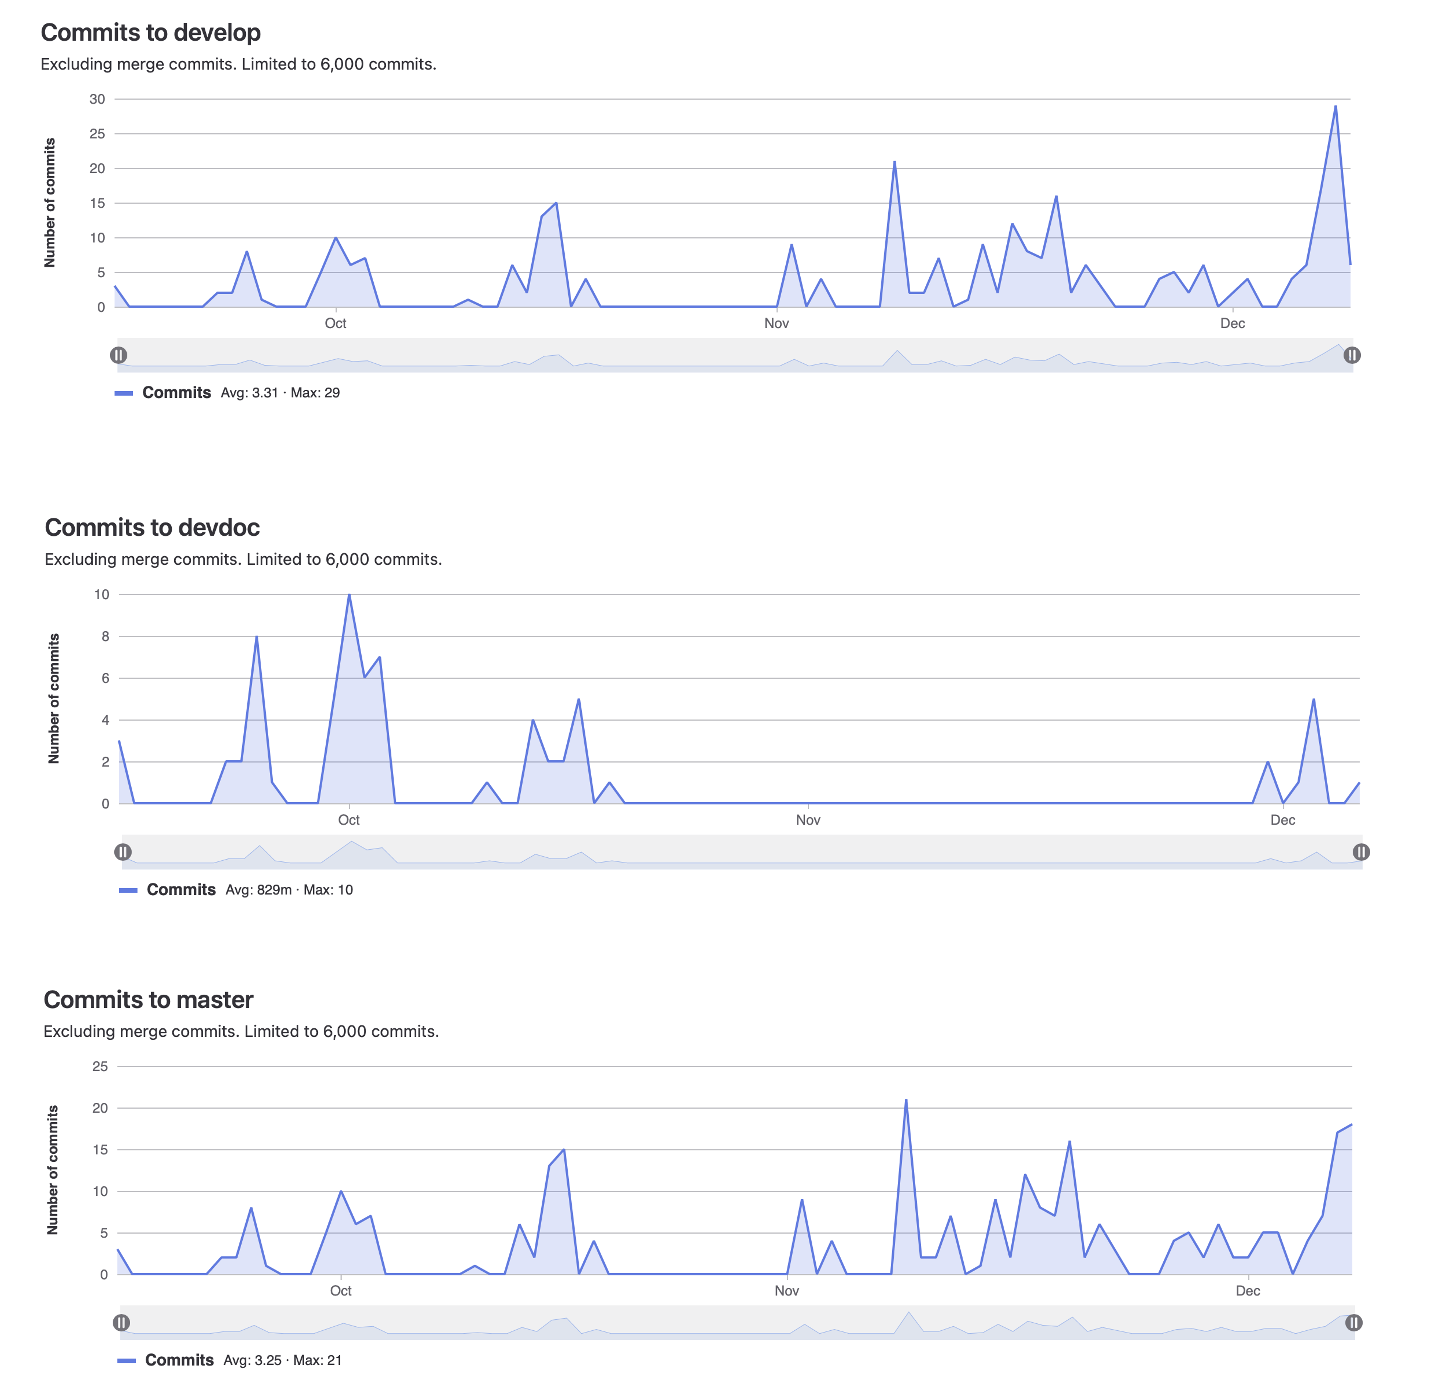
\includegraphics[width=\textwidth]{slike/dijagram_promjena.png}
			\caption{Dijagrami pregleda promjena nad datotekama izvornog koda i dokumentacije}
			\label{fig:my_label}
		\end{figure}
		
	